Durante la validaci\'on cruzada realizada para evaluar el rendimiento de los
distintos vectorizadores se fueron registrando varias m\'etricas de evaluaci\'on
para cada iteraci\'on como as\'i tambi\'en el tiempo de ajuste necesario en cada caso.
La figura \ref{fig-results-features-fit-time} muetra el promedio y el desv\'io
est\'andar de este \'ultimo en las cinco iteraciones realizadas. Como es posible
apreciar, el vectorizado de proporciones con remoci\'on de \textit{stopwords}
provenientes de \textit{NLTK} es el que presenta un tiempo de ajuste promedio
menor, y tambi\'en un menor desv\'io. El vectorizador de \textit{TF-IDF} con
frecuencia de documentos natural, por otro lado, es el que mayores valores
exhibe tanto en la media como en el desv\'io est\'andar. La tabla \ref{table-appendix-fit-time}
presente en la secci\'on \ref{appendix-table-vectorizers} del Anexo detalla una
a una las medidas de centralidad.

\begin{figure}[h!]
    \centering
    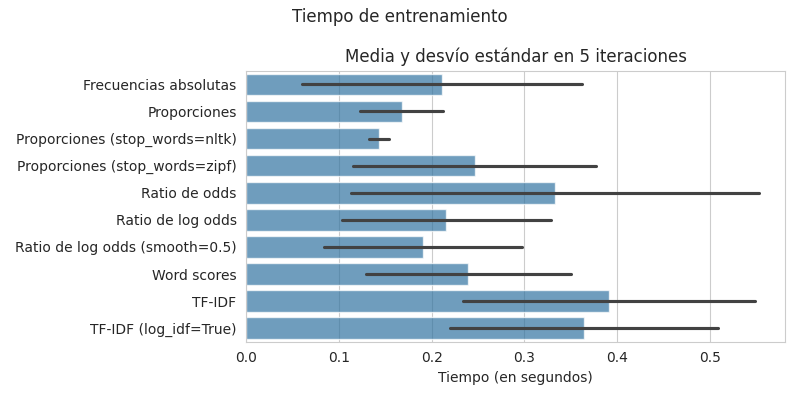
\includegraphics[scale=0.6]{../visualizations/features/fit_time.png}
    \caption{Media y desvi\'o est\'andar del tiempo de ajuste (medido en segundos)
    requerido para el entrenamiento de una regresi\'on log\'istica \textit{baseline}
    al utilizar distintos vecotrizadores siguiendo una estrategia de
    validaci\'on cruzada con cinco iteraciones.}
    \label{fig-results-features-fit-time}
\end{figure}

En cuanto a las m\'etricas de rendimiento,
la tabla \ref{table-results-vectorizers-val} ofrece el promedio de los valores
obtenidos en la validaci\'on cruzada para cada vectorizador. All\'i se puede ver que,
en la mayor\'ia de los casos, fue el vectorizador de \textit{TF-IDF} con logaritmo
de la frecuencia de documentos el que present\'o mejores resultados. Si bien el
vectorizador de proporciones con remoci\'on de \textit{stopwords} obtenidas por el
m\'etodo de Zipf se muestra superior a este en t\'erminos de precisi\'on, solo
lo hace a expensas de perder cobertura, lo que se conoce como la compensaci\'on o el
\textit{trade-off} entre ambas m\'etricas. De hecho, esta vectorizaci\'on es la que
presenta la peor cobertura de todos los m\'etodos evaluados. Y algo semejante ocurre
con el vectorizador basado en el \textit{ratio} de los \textit{log-odds} con
suavizado, que
muestra una mejor cobertura que el resto de los vectorizadores, pero una peor
precisi\'on, \textit{accuracy} y \textit{f1-macro}.

\begin{table}[h!]
    \centering
    \begin{adjustbox}{max width=\textwidth}
    \begin{tabular}{ *{7}{|c}| }
        \hline
        Vectorizador & \textit{Accuracy} & Precisi\'on & Cobertura & \textit{F1} & \textit{F1-weighted} & \textit{F1-macro} \\
        \hline\hline
        \makecell{Frecuencias\\absolutas} & 0.610 & 0.663 & 0.618 & 0.635 & 0.608 & 0.605 \\
        \hline
        Proporciones & 0.623 & 0.663 & 0.653 & 0.654 & 0.622 & 0.617 \\
        \hline
        \makecell{Proporciones\\($NLTK$)} & 0.623 & 0.663 & 0.653 & 0.654 & 0.622 & 0.617 \\
        \hline
        \makecell{Proporciones\\($Zipf$)} & 0.636 & \cellcolor{highlight-blue!60}0.726 & \cellcolor{highlight-orange!60}0.576 & 0.619 & 0.624 & 0.625 \\
        \hline
        \makecell{\textit{Ratio} de\\\textit{odds}} & 0.560 & 0.587 & 0.698 & \cellcolor{highlight-orange!60}0.611 & 0.518 & 0.506 \\
        \hline
        \makecell{\textit{Ratio} de\\\textit{log-odds}} & 0.560 & 0.587 & 0.698 & \cellcolor{highlight-orange!60}0.611 & \cellcolor{highlight-orange!60}0.451 & 0.506 \\
        \hline
        \makecell{\textit{Ratio} de\\\textit{log-odds}\\(suavizado)} & \cellcolor{highlight-orange!60}0.541 & \cellcolor{highlight-orange!60}0.555 & \cellcolor{highlight-blue!60}0.887 & 0.682 & 0.518 & \cellcolor{highlight-orange!60}0.419 \\
        \hline
        \textit{TF-IDF} & 0.572 & 0.595 & 0.731 & 0.630 & 0.521 & 0.506 \\
        \hline
        \makecell{\textit{TF-IDF}\\($log IDF$)} & \cellcolor{highlight-blue!60}0.667 & 0.699 & 0.721 & \cellcolor{highlight-blue!60}0.702 & \cellcolor{highlight-blue!60}0.663 & \cellcolor{highlight-blue!60}0.657 \\
        \hline
        \textit{Word scores} & 0.623 & 0.655 & 0.697 & 0.671 & 0.618 & 0.611 \\
        \hline
    \end{tabular}
    \end{adjustbox}
    \caption{Resultados obtenidos tras evaluar un modelo de
    regresi\'on log\'istica base utilizando
    vectorizadores basados en las distintas t\'ecnicas estad\'isticas.
    Los valores reflejan el rendimiento promedio de las cinco iteraciones
    de la validaci\'on cruzada.
    Las celdas resaltadas en azul corresponden a la estategia de vectorizaci\'on
    que obtuvo un mejor rendimiento promedio en cada
    m\'etrica de evaluaci\'on y las resaltadas en naranja, a la
    que obtuvo el peor rendimiento.}
    \label{table-results-vectorizers-val}
\end{table}

El vectorizador basado en \textit{TF-IDF (log IDF)} no solo presenta un mayor
\textit{accuracy} que el resto de las t\'ecnicas de vectorizaci\'on, sino que
tambi\'en muestra un mejor \textit{$F_{\beta}$ score} (con $\beta=1$).
Esta m\'etrica ofrece una representaci\'on sim\'etrica de la precisi\'on y la cobertura,
lo que nos indica que, si bien dicho vectorizador no es el que mejores valores
exhibe en estas m\'etricas, s\'i es el que mejor maneja la compensaci\'on
entre ambas. En este trabajo se decidi\'o utilizar $\beta=1$ porque no se busca
privilegiar ninguna de las dos por sobre la otra.
\par
Adicionalmente, se reportan el \textit{F1-macro} y \textit{F1-weighted}.
El primero consiste en un promedio del \textit{F1} calculado para ambas clases
predichas, lo que da una idea de la compensaci\'on de la precisi\'on y la
cobertura tomado en cuenta la clase $1$ (discursos positivos), por un lado, y
la clase $0$ (discursos negativos), por otro. No obstante, dado que ambas clases no
est\'an balancedas\footnote{Como se mencion\'o en la secci\'on
\ref{subsection-data-description}, el conjunto de datos presenta un $56\percentsign$
de discursos a favor y un $44\percentsign$ de discursos en contra.}, podr\'ia ser que,
al calcular el promedio, el buen rendimiento en la predicci\'on de una de las clases
enmascare la imperfecta predicci\'on de la otra. Es por esto
que tambi\'en se recurre al \textit{F1-weighted}, que multiplica el \textit{F1}
de cada clase por la proporci\'on de casos que esta presenta en el conjunto de datos,
de modo que el valor resultante es una medida ``pesada'' en relaci\'on a la representaci\'on
de cada clase. En la secci\'on \ref{appendix-plots-vectorizers} del Anexo pueden
apreciarse los gr\'aficos de estas m\'etricas para cada iteraci\'on de la validaci\'on
cruzada.
